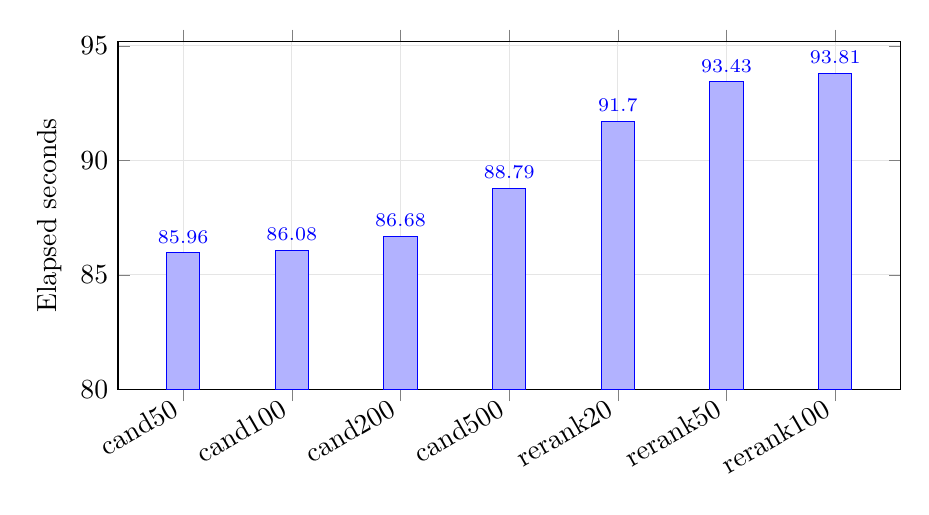
\begin{tikzpicture}
\begin{axis}[
  ybar,
  width=0.95\linewidth,
  height=6cm,
  ymin=80,
  ylabel={Elapsed seconds},
  symbolic x coords={cand50,cand100,cand200,cand500,rerank20,rerank50,rerank100},
  xtick=data,
  x tick label style={rotate=30, anchor=east},
  bar width=12pt,
  nodes near coords,
  nodes near coords align={vertical},
  every node near coord/.append style={font=\scriptsize},
  grid=major,
  grid style={draw=gray!20}
]
\addplot coordinates {
  (cand50,85.964)
  (cand100,86.081)
  (cand200,86.675)
  (cand500,88.789)
  (rerank20,91.702)
  (rerank50,93.427)
  (rerank100,93.807)
};
\end{axis}
\end{tikzpicture}
